\documentclass[a4paper, 12pt]{article}
\usepackage[top=1.5cm, bottom=1.5cm, left=1.5cm, right=1.5cm]{geometry}
\usepackage{float}
\usepackage[utf8]{inputenc}
\usepackage{array}
\usepackage{geometry}
\usepackage{placeins}
\usepackage{pgfplots}
\pgfplotsset{compat=1.18}

\begin{document}
	\begin{center}
		Universidade Federal do Rio Grande do Norte
		
		Departamento de Engenharia da Computação e Automação  
		
		DCA3703 - Programação Paralela  
		
		\textbf{Tarefa 13: Afinidade de threads}  
		
		\textbf{Aluno:} Daniel Bruno Trindade da Silva  
	\end{center}  
	
	\section{Introdução}
	
	\hspace{0.62cm}Este relatório tem como objetivo apresentar os conhecimentos adquiridos durante a realização da Tarefa 13 da disciplina de \textbf{Computação Paralela}. A atividade consistiu em avaliar a escalabilidade do programa desenvolvido na Tarefa 11 — um simulador da velocidade de um fluido utilizando a equação de Navier-Stokes — aplicando diferentes políticas de afinidade de \textit{threads}.
	
	\section{Enunciado}
	
	\hspace{0.62cm}Avalie como a escalabilidade do seu código de Navier-Stokes muda ao utilizar os diversos tipos de afinidades de \textit{threads} suportados pelo sistema operacional e pelo OpenMP, no mesmo nó de computação do NPAD utilizado para a Tarefa 12.
	
	\section{Desenvolvimento}
	
	\hspace{0.62cm}Na Tarefa 11, desenvolvemos duas versões de um programa para simular a velocidade de um fluido: uma versão sequencial (serial) e outra paralelizada com OpenMP. Para a análise requerida nesta tarefa, utilizamos a versão paralelizada do código.
	
	\hspace{0.62cm}Nesta tarefa, analisamos os impactos da cláusula \texttt{proc\_bind()} com as seguintes políticas de afinidade:
	
	\begin{itemize}
		\item \textbf{\texttt{spread}} — O openMP distribui as \textit{threads} de forma espalhada pelos processadores, maximizando a distância entre elas. O objetivo é utilizar o máximo de recursos do hardware possível, como diferentes \textit{sockets} ou núcleos físicos. Aumenta a latência de comunicação entre as \textit{threads} em troca de menos disputa por recurso. Ideal quando temos programas com \textit{threads} independentes;
		
		\item \textbf{\texttt{close}} — O openMP agrupa as \textit{threads} próximas umas das outras, preferencialmente no mesmo \textit{socket} ou núcleos adjacentes ao da \textit{thread} master. Utilizada quando queremos manter as \textit{threads} próximas pra diminuir a latência, mas não queremos sobrecarregar um mesmo núcleo;
		
		\item \textbf{\texttt{master}} — Nessa política todas as \textit{threads} são alocadas no mesmo local onde a \textit{thread} principal (\textit{master/primary}) está executando. Utilizado quando a comunicação entre \textit{threads} é muito intensa e isso compença a perda de paralelismo. Pois ela gera disputa por recursos, mas reduz a latência de comunicação entre as \textit{threads};
		
		\item \textbf{\texttt{true}} — herda a política de afinidade da região paralela pai. Se não houver região pai, comporta-se de acordo com a política padrão definida pela implementação.
		
		\item \textbf{\texttt{false}} — Desativa a afinidade de \textit{threads} o escalonador do sistema operacional é quem vai decidir onde cada \textit{thread} ficará. Com isso pode haver migração de \textit{threads} entre núcleos causando mais overhead e menos previsibilidade;
	\end{itemize}
	
	Reorganizamos o código de forma a possibilitar o teste de todas as políticas em uma única execução. Assim como realizado na Tarefa 12, o código foi executado com 1, 2, 4, 8, 16 e 32 \textit{threads}, para que ao final pudéssemos analisar se houve influência dessas políticas de afinidade na eficiência do código.
	
	O código foi executado no super computador da universidade utilizando o nó com o processador intel-128, cada teste foi executado 6 vezes para termos a certeza da constância dos resultados.
	
	\section{Resultados}
	\hspace{0.62cm}Iniciaremos avaliando a escalabilidade forte fixando o tamanho de nosso problema e aumentando o número de threads utilizados para o processamento. A figura abaixo mostra nossos resultados: 
	
	\begin{center}
		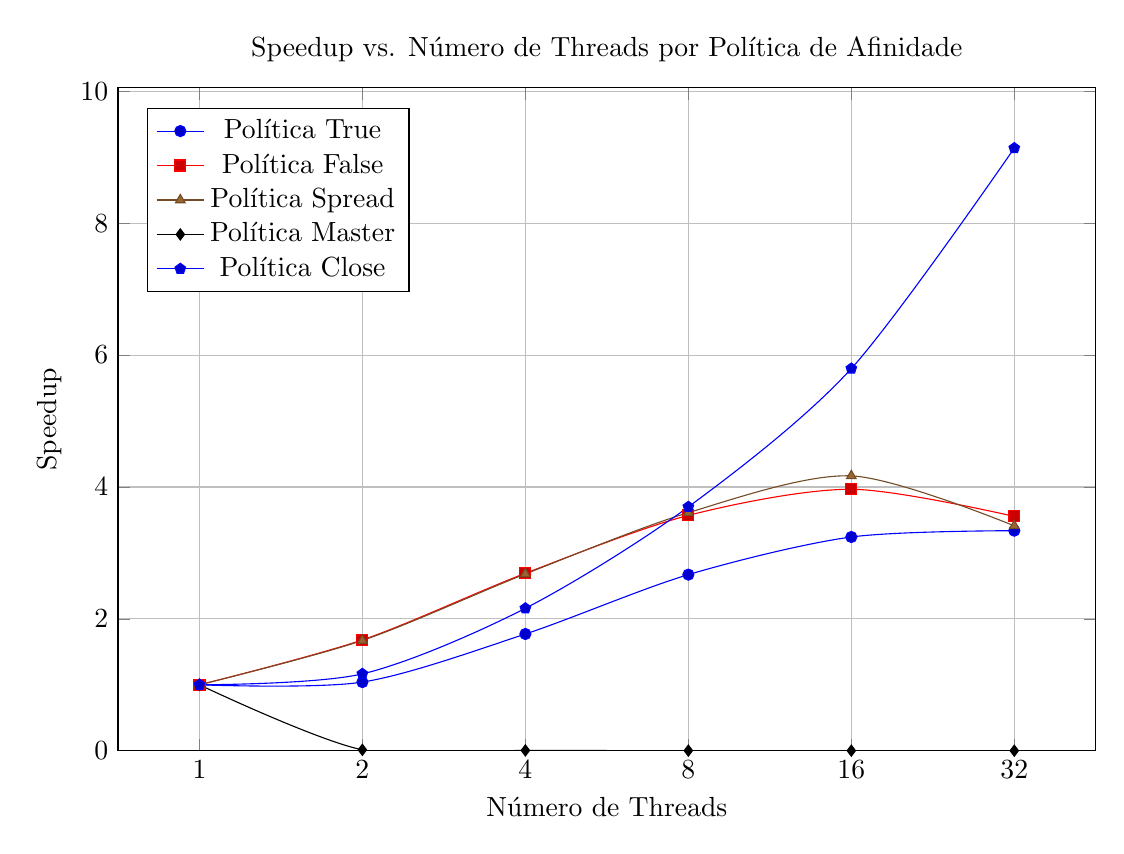
\begin{tikzpicture}
			\begin{axis}[
				title={Speedup vs. Número de Threads por Política de Afinidade},
				xlabel={Número de Threads},
				ylabel={Speedup},
				xmode=log,                      % Eixo X em escala logarítmica
				log ticks with fixed point,     % Formato dos ticks no eixo log
				xtick={1,2,4,8,16,32},
				xticklabels={1,2,4,8,16,32},
				legend pos=north west,          % Posição da legenda
				grid=major,                     % Adiciona grade principal
				width=14cm,                     % Largura do gráfico
				height=10cm,                    % Altura do gráfico
				ymin=0,                         % Valor mínimo do eixo Y
				% ymax pode ser ajustado conforme necessário, mas pgfplots geralmente lida bem automaticamente
				]
				
				% Dados para o gráfico
				% Politica True
				\addplot+[mark=*, smooth] coordinates {
					(1, 1.000000) (2, 1.041223) (4, 1.770291) (8, 2.670522) (16, 3.241188) (32, 3.337166)
				};
				\addlegendentry{Política True}
				
				% Politica False
				\addplot+[mark=square*, smooth] coordinates {
					(1, 1.000000) (2, 1.681153) (4, 2.691582) (8, 3.568715) (16, 3.965107) (32, 3.553509)
				};
				\addlegendentry{Política False}
				
				% Politica Spread
				\addplot+[mark=triangle*, smooth] coordinates {
					(1, 1.000000) (2, 1.672246) (4, 2.680801) (8, 3.610364) (16, 4.168062) (32, 3.410142)
				};
				\addlegendentry{Política Spread}
				
				% Politica Master
				\addplot+[mark=diamond*, smooth] coordinates {
					(1, 1.000000) (2, 0.014110) (4, 0.004771) (8, 0.002045) (16, 0.000951) (32, 0.000461)
				};
				\addlegendentry{Política Master}
				
				% Politica Close
				\addplot+[mark=pentagon*, smooth] coordinates {
					(1, 1.000000) (2, 1.165592) (4, 2.160008) (8, 3.698040) (16, 5.795370) (32, 9.137857)
				};
				\addlegendentry{Política Close}
				
			\end{axis}
		\end{tikzpicture}
	
	\end{center}
	
	Na figura abaixo temos o mesmo gráfico, mas com a curva do \textit{speedup} ideal para fins de comparação
		
	\begin{center}
	
		
		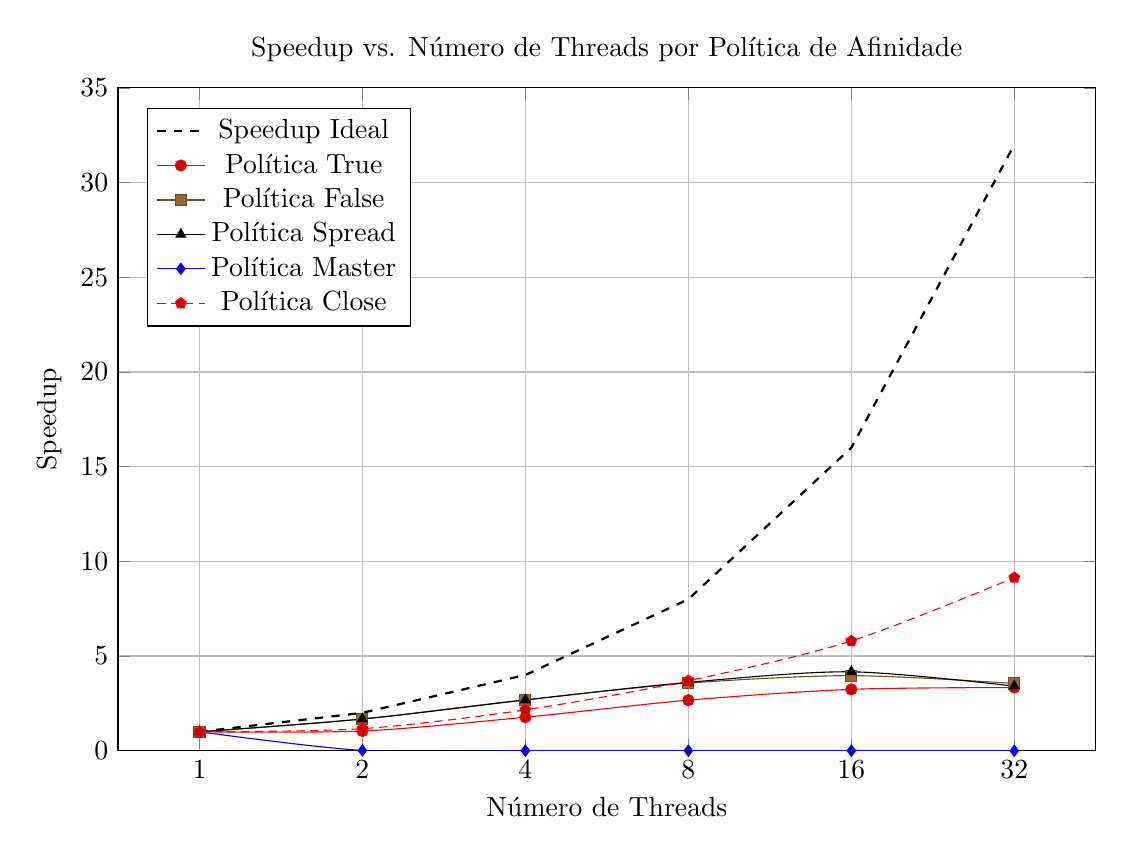
\begin{tikzpicture}
			\begin{axis}[
				title={Speedup vs. Número de Threads por Política de Afinidade},
				xlabel={Número de Threads},
				ylabel={Speedup},
				xmode=log,                      % Eixo X em escala logarítmica
				log ticks with fixed point,     % Formato dos ticks no eixo log
				xtick={1,2,4,8,16,32},
				xticklabels={1,2,4,8,16,32},
				legend pos=north west,          % Posição da legenda
				grid=major,                     % Adiciona grade principal
				width=14cm,                     % Largura do gráfico
				height=10cm,                    % Altura do gráfico
				ymin=0,                         % Valor mínimo do eixo Y
				ymax=35,                        % Ajustado para incluir o speedup ideal de 32
				]
				
				% Curva de Speedup Ideal
				\addplot+[mark=none, dashed, thick, color=black] coordinates {
					(1, 1) (2, 2) (4, 4) (8, 8) (16, 16) (32, 32)
				};
				\addlegendentry{Speedup Ideal}
				
				% Dados para o gráfico - Políticas Reais
				% Politica True
				\addplot+[mark=*, smooth] coordinates {
					(1, 1.000000) (2, 1.041223) (4, 1.770291) (8, 2.670522) (16, 3.241188) (32, 3.337166)
				};
				\addlegendentry{Política True}
				
				% Politica False
				\addplot+[mark=square*, smooth] coordinates {
					(1, 1.000000) (2, 1.681153) (4, 2.691582) (8, 3.568715) (16, 3.965107) (32, 3.553509)
				};
				\addlegendentry{Política False}
				
				% Politica Spread
				\addplot+[mark=triangle*, smooth] coordinates {
					(1, 1.000000) (2, 1.672246) (4, 2.680801) (8, 3.610364) (16, 4.168062) (32, 3.410142)
				};
				\addlegendentry{Política Spread}
				
				% Politica Master
				\addplot+[mark=diamond*, smooth] coordinates {
					(1, 1.000000) (2, 0.014110) (4, 0.004771) (8, 0.002045) (16, 0.000951) (32, 0.000461)
				};
				\addlegendentry{Política Master}
				
				% Politica Close
				\addplot+[mark=pentagon*, smooth] coordinates {
					(1, 1.000000) (2, 1.165592) (4, 2.160008) (8, 3.698040) (16, 5.795370) (32, 9.137857)
				};
				\addlegendentry{Política Close}
				
			\end{axis}
		\end{tikzpicture}
	\end{center}
		
	\section{Analise dos Resultados}
	
	As politicas de afinidade de \textit{thread} foram testadas na sequencia em que as tabelas foram montadas. Essas tabelas mostram o comportamento da escalabilidade relacionando o tamanho do problema com a quantidade de \textit{thread} que a executaram, medindo através da sua eficiência.
	
	\subsection{Spread, True e Close}
	Essas três políticas apresentaram comportamentos muito similares, caracterizados por eficiências bastante baixas em praticamente todas as configurações. A eficiência caiu rapidamente com o aumento do número de threads, atingindo valores próximos a zero com 16 e 32 threads. O aumento do tamanho do problema trouxe pouca ou nenhuma melhora significativa na eficiência, indicando baixa escalabilidade fraca.
	
	\subsection{Master}
	A política MASTER apresentou a pior eficiência dentre todas as políticas avaliadas. Com 2 e 4 threads, as eficiências foram próximas de zero. Apenas a partir de 8 threads observou-se alguma melhora, embora ainda em níveis muito baixos (em torno de 0,11 a 0,12). A ampliação do tamanho do problema não resultou em ganhos expressivos.
	
	Esse resultado era totalmente esperado, uma vez que essa política centraliza a execução na thread principal, criando um gargalo que impede a distribuição eficiente da carga de trabalho. Assim, a política MASTER é reconhecidamente inadequada para programas paralelos que visam alta escalabilidade, conforme foi comprovado experimentalmente
	
	\subsection{False}
	Esta política apresentou as melhores eficiências gerais em todas as configurações, especialmente com 2 e 4 threads, onde atingiu valores próximos a 0,9, indicando bom aproveitamento do paralelismo. Apesar de a eficiência cair progressivamente com o aumento do número de threads, ela se manteve superior às demais políticas. O aumento do tamanho do problema resultou em melhoras discretas na eficiência, evidenciando um comportamento típico de escalabilidade fraca.
	
	Era esperado que a ausência de afinidade permitisse ao sistema operacional otimizar a distribuição das threads, minimizando contenções e promovendo melhor balanceamento de carga. De fato, isso foi confirmado pelos resultados. O desempenho atendeu às expectativas.
	
	\section{Conclusão}

	A análise realizada demonstrou que as políticas de afinidade de threads exercem um impacto significativo na eficiência e escalabilidade de programas paralelos. Os experimentos confirmaram que a escolha inadequada da política pode comprometer substancialmente o desempenho da aplicação.
	
	De forma geral, os resultados obtidos foram coerentes com a literatura e com o comportamento esperado para cada política, destacando a necessidade de uma análise criteriosa do perfil computacional de cada aplicação antes de definir a política de afinidade de threads. A escalabilidade forte se mostrou limitada em todas as políticas quando o número de threads foi elevado excessivamente, enquanto a escalabilidade fraca apresentou melhoras modestas, especialmente na política FALSE.
	
	Por fim, esta avaliação reforça a importância de realizar experimentos empíricos para orientar decisões de configuração em sistemas paralelos, visando sempre o melhor aproveitamento dos recursos computacionais disponíveis.
	
	

	 

\end{document}
